\newpage

\section{Another option for the instrumental distribution in the Accept-Reject algorithm is to use another beta distribution. Since we saw before how to simulate random values from a beta distribution for which the shape parameters take on natural values, we will use this kind of beta distribution.}


% -------------------------------------------------------------------------------------------------

\subsection*{(a) Show formally that, for the ratio $f/g$ to be bounded when $f$ is a $\text{Be}(\alpha, \beta)$ density and $g$ is a $\text{Be}(a, b)$ density, we must have both $a \leq \alpha$ and $b \leq \beta$. Determine the maximal ratio in terms of $\alpha$, $\beta$, $a$, and $b$.}

Let \(f(x)\) and \(g(x)\) be the probability density functions of \(\text{Be}(\alpha, \beta)\) and \(\text{Be}(a, b)\), respectively:
\begin{equation}
f(x) = \frac{1}{B(\alpha, \beta)} x^{\alpha - 1} (1 - x)^{\beta - 1}, \quad x \in [0,1]
\end{equation}
\begin{equation}
g(x) = \frac{1}{B(a, b)} x^{a - 1} (1 - x)^{b - 1}, \quad x \in [0,1]
\end{equation}

Consider the ratio of densities:
\begin{align}
\frac{f(x)}{g(x)} &= \frac{\frac{1}{B(\alpha, \beta)} x^{\alpha - 1} (1 - x)^{\beta - 1}}{\frac{1}{B(a, b)} x^{a - 1} (1 - x)^{b - 1}} \\
&= \frac{B(a, b)}{B(\alpha, \beta)} \cdot x^{\alpha - a} (1 - x)^{\beta - b}
\end{align}

Since the support is the interval \([0,1]\), for the ratio \(\frac{f}{g}\) to be bounded on \([0,1]\), the powers of \(x\) and \((1 - x)\) must not cause divergences at the boundaries:
\begin{itemize}
    \item If \(\alpha - a < 0\), then \(x^{\alpha - a} \to \infty\) as \(x \to 0\).
    \item If \(\beta - b < 0\), then \((1 - x)^{\beta - b} \to \infty\) as \(x \to 1\).
\end{itemize}
Hence, to avoid unbounded behavior: $\alpha - a \geq 0 \text{ and } \beta - b \geq 0 \Rightarrow a \leq \alpha,\ b \leq \beta$


\vspace{1em}
\textbf{Finding the maximum of the ratio}

Define:
\begin{equation}
h(x) = x^{\alpha - a} (1 - x)^{\beta - b}, \quad x \in (0,1)
\end{equation}

The derivative is:
\begin{align}
h'(x) &= (\alpha - a) x^{\alpha - a - 1} (1 - x)^{\beta - b} - (\beta - b) x^{\alpha - a} (1 - x)^{\beta - b - 1} \\
&= x^{\alpha - a - 1} (1 - x)^{\beta - b - 1} \left[ (\alpha - a)(1 - x) - (\beta - b) x \right]
\end{align}

The critical points satisfy:
\begin{equation}
(\alpha - a)(1 - x) - (\beta - b) x = 0 \quad \Rightarrow \quad x = \frac{\alpha - a}{\alpha - a + \beta - b}
\end{equation}

The maximum of the ratio \(\frac{f}{g}\) is attained at this point:
\[
C = \max_{x \in [0,1]} \frac{f(x)}{g(x)} = \frac{B(a, b)}{B(\alpha, \beta)} \left( \frac{\alpha - a}{\alpha - a + \beta - b} \right)^{\alpha - a} \left( \frac{\beta - b}{\alpha - a + \beta - b} \right)^{\beta - b}
\]

This constant \(C\) serves as the limiting constant in the Accept–Reject algorithm when using \(\text{Be}(a,b)\) as instrumental to sample from \(\text{Be}(\alpha, \beta)\).





% please update the python implementation for part (b) based on updated part (a)
% please help me provide the answer for part (b)


% ---

% We want to show that $a \leq \alpha$ and $b \leq \beta$ must be true for the ratio $\frac{f}{g}$ to be bounded. Replacing $f$ and $g$ by their definitions of the PDF of a beta distribution, we have

% \[
% \frac{f(x)}{g(x)} = \frac{\dfrac{B(a, b)}{B(\alpha, \beta)} \cdot \dfrac{x^{\alpha - 1}}{x^{a - 1}} \cdot \dfrac{(1 - x)^{\beta - 1}}{(1 - x)^{b - 1}}}
% = \frac{B(a, b)}{B(\alpha, \beta)} \cdot x^{\alpha - a} \cdot (1 - x)^{\beta - b}
% \]

% Since $x$ is between 0 and 1, the term $x^{\alpha - a}$ explodes if $\alpha - a < 0$ (for small value of $x$, close to 0). The term $(1 - x)^{\beta - b}$ explodes if $\beta - b < 0$ (for big value of $x$, close to 1). To avoid that such terms explode, we have to ensure that $a \leq \alpha$ and $b \leq \beta$.

% \vspace{0.5em}

% We can determine the maximal ratio $\frac{f}{g}$ by canceling its derivative:
% \[
% \frac{\delta}{\delta x} \left( \frac{f(x)}{g(x)} \right) = 0
% \]

% \[
% \frac{\delta}{\delta x} \left( \frac{B(a,b)}{B(\alpha, \beta)} \cdot x^{\alpha - a} \cdot (1 - x)^{\beta - b} \right) = 0
% \]

% Since $\frac{B(a,b)}{B(\alpha,\beta)}$ is constant for given $a$, $b$, $\alpha$ and $\beta$, we can write:

% \[
% \frac{\delta}{\delta x} \left( x^{\alpha - a} (1 - x)^{\beta - b} \right) = 0
% \]

% \vspace{0.5em}
% The derivative can be computed:

% \[
% (\alpha - a)x^{\alpha - a - 1}(1 - x)^{\beta - b} - (\beta - b)x^{\alpha - a}(1 - x)^{\beta - b - 1} = 0
% \]

% \[
% x^{\alpha - a - 1}(1 - x)^{\beta - b - 1} \left[ (\alpha - a)(1 - x) - (\beta - b)x \right] = 0
% \]

% There is an extremum at $x_1 = 0$, $x_2 = 1$ and 
% \[
% x_3 = \frac{\alpha - a}{\alpha - a + \beta - b}
% \]
% The maximum value is at $x_3$.




% -------------------------------------------------------------------------------------------------
% \newpage
\subsection*{(b) Redo questions 7(b) to 7(d) with the appropriate beta distribution as instrumental distribution. Compare both methods.}

% We now apply the Accept–Reject algorithm using a Beta distribution as instrumental density. Specifically, we use \( g(x) = \text{Be}(3, 9) \) to generate samples from the target distribution \( f(x) = \text{Be}(3.3, 9.5) \). This choice satisfies the condition \( a \leq \alpha \), \( b \leq \beta \), ensuring that the ratio \( f/g \) is bounded on \([0,1]\).

% \vspace{0.5em}
% \textbf{Compute the limiting constant \( C \)}

The density ratio is:
\begin{equation}
\frac{f(x)}{g(x)} = \frac{B(3, 9)}{B(3.3, 9.5)} \cdot x^{0.3} (1 - x)^{0.5}    
\end{equation}

with its maximum at:
\[
x_{\max} = \frac{\alpha - a}{\alpha - a + \beta - b} = \frac{3.3 - 3}{(3.3 - 3) + (9.5 - 9)} = \frac{0.3}{0.8} = 0.375
\]

Evaluating the ratio at \(x_{\max}\) yields the limiting constant:
\[
C \approx 1.0761
\]

We performed Accept–Reject sampling until exactly \(n = 15,000\) accepted values were obtained. The empirical acceptance rate was:
\[
\text{Acceptance rate} = \frac{\text{\# accepted}}{\text{\# accepted} + \text{\# rejected}} = \frac{\text{\# accepted}}{15,\!000} \approx 92.99\%
\]

Figure~\ref{fig:8b} shows the histogram of accepted and rejected samples, along with the true Beta(3.3, 9.5) density and the instrumental Beta(3, 9) density.

\begin{figure}[H]
    \centering
    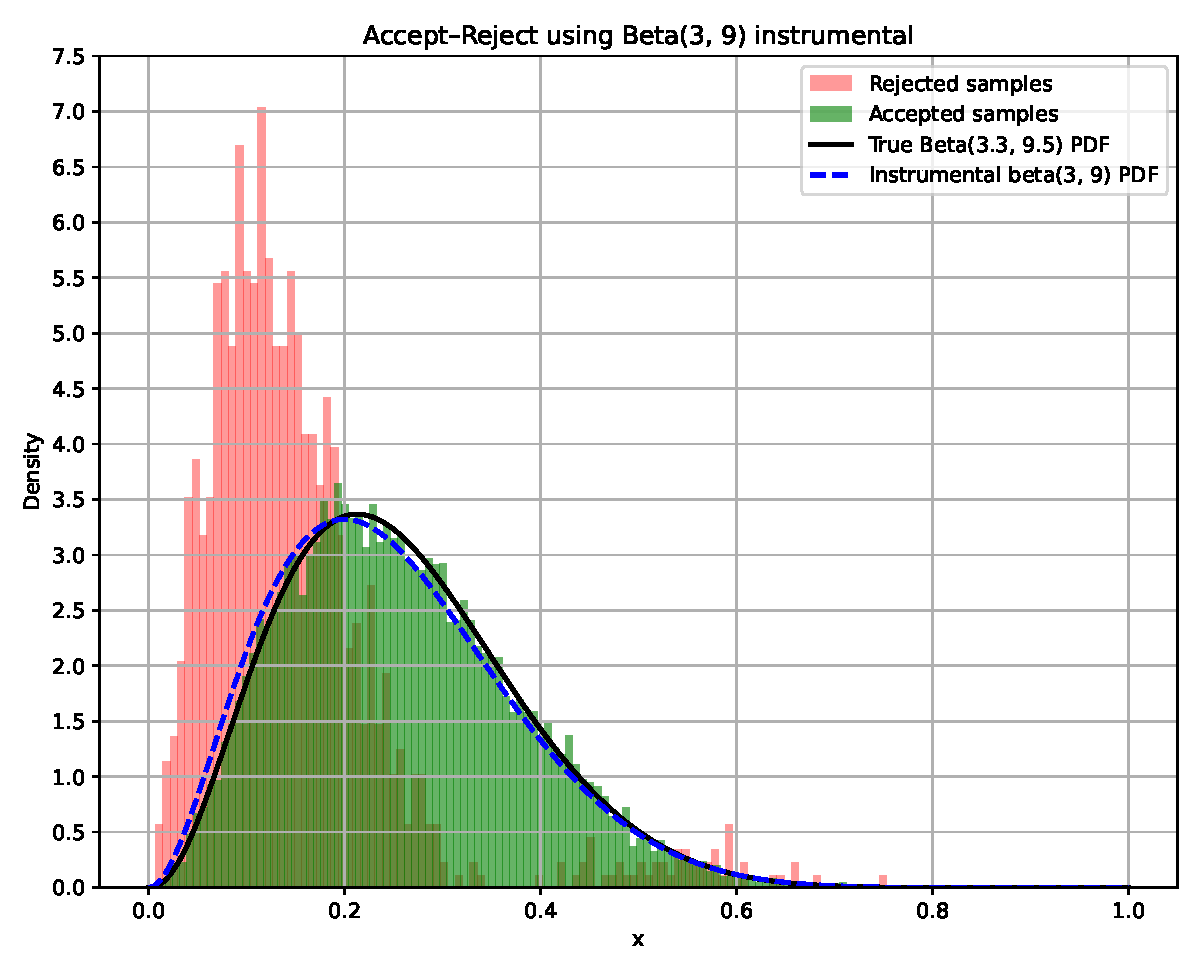
\includegraphics[width=0.7\textwidth]{resources/figures/q8b-beta_instrumental.pdf}
    \noskipcaption{Accept–Reject using Beta(3, 9) as instrumental distribution for sampling from Beta(3.3, 9.5).}
    \label{fig:8b}
\end{figure}

\begin{itemize}
    \item Acceptance rate: Using Beta(3, 9) as the instrumental distribution results in a significantly higher acceptance rate (92.99\%) compared to the uniform instrumental method (29.41\%).
    \item Efficiency: Selecting an instrumental distribution close to the target greatly reduces the number of rejected samples, improving computational efficiency.
    \item Simulation quality: The accepted samples closely match the true Beta distribution, validating the effectiveness of this approach.
\end{itemize}



% \vspace{0.5em}
% \textbf{Conclusion:} Using a Beta distribution as the instrumental density is clearly more efficient and yields higher quality samples than using a uniform distribution, especially when the chosen instrumental parameters closely resemble those of the target distribution.




% ---

% The acceptance rate is equal to 0.7168, which is way higher when using the uniform distribution as instrumental density. The limiting constant $C$ is equal to 1.3994. The plot of the accepted samples and rejected samples is displayed below.

% \begin{figure}[h]
%     \centering
%     % \includegraphics[width=0.8\textwidth]{your-figure-file.pdf} % Replace with actual figure filename
%     \caption{Accept-Reject algorithm for beta distribution with beta distribution as instrumental density (10,000 samples).}
%     \label{fig:accept-reject-beta-instrument}
% \end{figure}

% We can interpret the limiting constant $C$ as the number of samples needed on average before accepting a sample. Using this definition, we can understand that the choice of the instrumental density is crucial. Indeed, the efficiency of the method is highly dependent on that choice. When using the uniform distribution as instrumental density, the limiting constant $C$ was equal to 3.5864, while when using a beta distribution, the $C$ constant is equal to 1.3994. It basically means that we nearly need 3 times more samples to have the same number of accepted values.

% The percentage, which is linked to the limiting constant, is maybe more "understandable": using the uniform distribution, we had 27.88\% chance of accepting a sample, while using the beta distribution, we have 71.68\%. Therefore, using the beta distribution is highly efficient compared with using the uniform distribution. The Accept-Reject method is then more effective when the instrumental distribution resembles the target distribution (which clearly is the case in our example).

